\chapter{Dataset Selection and Analysis}
\label{ch:data}

\section{Why these datasets}
The project brief prescribes MiliPoint (primary) and RadHAR (secondary). Both are
public, both are produced by Texas Instruments single-chip radars, and both
provide point clouds rather than spectrograms. Together they cover two
complementary regimes. MiliPoint is a large benchmark (49 actions, 11 subjects)
that records \emph{who} performed each sequence, which makes a subject-disjoint
split possible. RadHAR is small (5 activities) but provides Doppler and intensity
for every point and an official test partition used by most prior work.

\textbf{Alternatives considered.} MM-Fi \cite{yang2023mmfi} (multi-modal, 27
actions) and mmBody \cite{chen2022mmbody} (mesh reconstruction) were reviewed.
MM-Fi is large (tens of GB), is aimed at multi-modal fusion and needs a separate
access request. mmBody has no activity labels. Neither was required by the brief,
so neither was used. No dataset was replaced.

\section{Availability and licences}
\begin{table}[h]
\centering
\caption{Dataset availability.}
\label{tab:avail}
\small
\begin{tabular}{L{2.2cm}L{5.5cm}L{2.6cm}L{4.0cm}}
\toprule
Dataset & Source & Licence & Access in this project \\
\midrule
RadHAR & github.com/nesl/RadHAR (raw data in repository) & BSD-3-Clause & \texttt{git clone}, 975\,MB \\
MiliPoint & github.com/yizzfz/MiliPoint (code, \texttt{id.json}); data zip on Google Drive & MIT & Drive blocked by the network proxy; zip downloaded manually by the team and staged (Issue \#3) \\
\bottomrule
\end{tabular}
\end{table}

\section{Data format and acquisition}
\textbf{RadHAR.} Raw files are text dumps of ROS \texttt{PointCloud} messages,
with one message per detected point (\texttt{seq}, timestamp, \texttt{point\_id},
$x,y,z$, range, velocity, Doppler bin, bearing, intensity). A new radar frame
starts whenever \texttt{point\_id} resets to 0. The radar is a TI IWR1443 using
the \texttt{ti\_mmwave\_rospkg} driver. The dataset paper reports two subjects,
but the files carry no subject identifier.

\textbf{MiliPoint.} Nineteen pickle files, each a list of frames with
\texttt{x} (points $[n,3]$) and \texttt{y} (18 pose keypoints), plus a global
\texttt{action\_label.npy} (one label per frame; $-1$ = unlabelled) and
\texttt{id.json} mapping the 11 subjects to files. The radar is a TI IWR1843 at
24 frames per second; subjects followed an instructional video of 49 actions of
30\,s each \cite{cui2023milipoint}. Action \emph{names} are not distributed with
the data, so actions are referred to by their numeric ID (0--48).

\section{Measured characteristics}
\begin{table}[h]
\centering
\caption{Dataset characteristics measured by \texttt{scripts/eda.py}.}
\label{tab:datachar}
\small
\begin{tabular}{L{4.6cm}L{4.6cm}L{4.6cm}}
\toprule
 & RadHAR & MiliPoint \\
\midrule
Subjects & 2 (paper); IDs not available & 11 (IDs available) \\
Classes & 5: boxing, jumping jacks, jump, squats, walk & 49 actions (IDs 0--48) \\
Recordings & 200 (142 train, 58 test) & 19 session files; 1{,}139 single-action runs \\
Duration / frames & 71.5 min train + 21.4 min test & 545{,}059 frames; 212{,}920 labelled \\
Frame rate & 30\,Hz nominal (irregular timestamps) & 24\,Hz \\
Points per frame (median / mean) & 21 / 21.4 & 6 / 6.5 \\
Point features & $x,y,z$, Doppler (quantised), intensity & $x,y,z$ only \\
Coordinate frame & $x$ forward, $y$ lateral, $z$ up & $x$ lateral, $y$ forward, $z$ up (verified from keypoints) \\
Missing / corrupted & none found; 34.6\% antenna self-returns & file 4 fully unlabelled; files 1, 6 partly \\
\bottomrule
\end{tabular}
\end{table}

\begin{figure}[h]
\centering
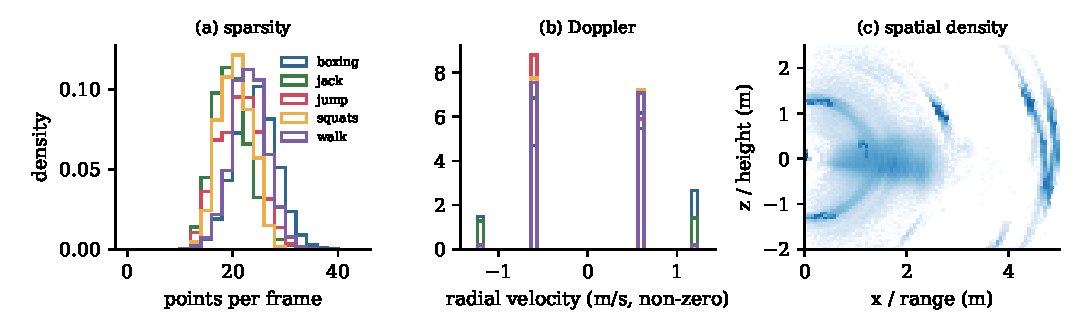
\includegraphics[width=\textwidth]{eda_radhar.pdf}
\caption{RadHAR. (a) points per frame by class; (b) non-zero Doppler values, which take only a few quantised values ($\pm0.6$, $\pm1.2$\,m/s); (c) density of all returns in the range--height plane (log scale): the person sits at 1--2\,m, and static clutter bands lie at about 2.5\,m and 4.5\,m.}
\label{fig:edarh}
\end{figure}

\begin{figure}[h]
\centering
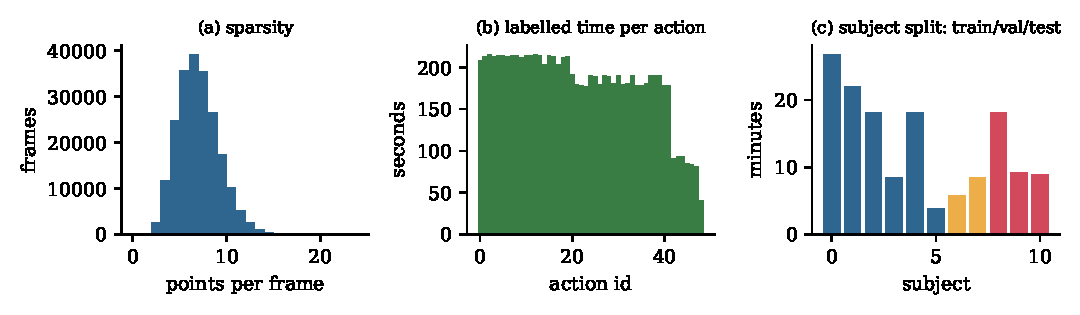
\includegraphics[width=\textwidth]{eda_milipoint.pdf}
\caption{MiliPoint. (a) points per frame (median 6); (b) labelled time per action; (c) labelled minutes per subject and the subject-disjoint split (blue train, orange validation, red test).}
\label{fig:edamp}
\end{figure}

\begin{figure}[h]
\centering
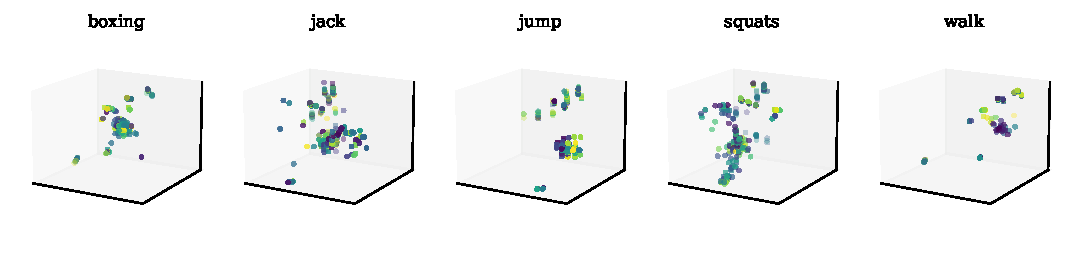
\includegraphics[width=\textwidth]{radhar_examples.pdf}
\caption{One pre-processed 2-s RadHAR test window per class (points coloured by time).}
\label{fig:rhex}
\end{figure}

\section{Class distribution}
RadHAR training recordings per class (boxing, jack, jump, squats, walk) are
26/28/26/29/33 and test recordings 13/10/11/10/14. The test windows per class
are 714/673/734/674/770, which is close to balanced. Some training recordings
are much longer than the standard 20\,s (for example \texttt{boxing\_184s.txt}
and \texttt{\_\_\_squats\_186s.txt}). This turned out to matter for validation
(Issue \#16--\#17). MiliPoint actions 0--40 have about 200\,s of labelled data
each, and actions 41--48 fewer (Fig.~\ref{fig:edamp}b).

\section{Noise characteristics (measured, not assumed)}
\begin{itemize}[nosep]
\item \textbf{Antenna self-returns}: 34.6\% of RadHAR returns lie at $x<0.3$\,m.
\item \textbf{Static clutter / multipath}: after the ROI filter, 50.1\% of returns lie more than
  1.2\,m (horizontally) from the moving-point centre of the person. They form
  persistent clusters at fixed ranges with zero Doppler (Fig.~\ref{fig:preprocreport}).
\item \textbf{Sparsity and variable density}: 15--28 returns per frame (5th--95th
  percentile) on RadHAR, and a median of 6 on MiliPoint.
\item \textbf{Doppler quantisation}: velocities take a handful of discrete values.
\item \textbf{Not observed}: corrupted files, NaN values or duplicated recordings
  (verified by the leakage audit, Chapter~\ref{ch:leak}).
\end{itemize}
Random coordinate displacement, point dropout, false detections and frame loss
are \emph{not} directly measurable without ground-truth body surfaces. They are
therefore studied as \emph{controlled synthetic perturbations} of recorded data
(Chapter~\ref{ch:pre}), and are clearly distinguished from the measured noise
above.

\section{Can the datasets be combined?}
Not as one training set. The label sets differ (5 vs 49 classes, and MiliPoint
action names are not published, so no reliable label mapping exists). The radars
differ (IWR1443 vs IWR1843), MiliPoint lacks Doppler and intensity, and the axes
differ. We therefore run \textbf{independent experiments} per dataset and use the
other dataset only for \textbf{representation transfer} after harmonising the
axes and restricting the input to $xyz$ (Chapter~\ref{ch:results}).

\section{Existing evaluation protocols}
RadHAR: an official train/test partition by recording, with validation on a
random 20\% of training \emph{windows} (which overlap by 50/60 frames).
MiliPoint: the published code concatenates labelled frames from all files and
cuts them chronologically 80/10/10, so the test data contain subjects that also
appear in training; other work uses random 80/10/10 splits \cite{zakka2025makgcn}.
Chapter~\ref{ch:leak} measures the leakage of each protocol.

\section{Dataset limitations}
RadHAR has no subject IDs and only two subjects. Its official test recordings were
made on the same days as the training recordings, often minutes apart
(Chapter~\ref{ch:leak}). MiliPoint provides $xyz$ only, and its action names are
unknown. Neither dataset contains falls or multi-person scenes.
